\documentclass{beamer}
\usepackage{inconsolata,fancyvrb,listings}

\newcommand{\ccft}[3]{
\usebeamercolor{#1}
\definecolor{#2}{named}{fg}
\definecolor{#3}{named}{bg}
}

\ccft{block title}{myblock title fg}{myblock title bg}
\ccft{block body}{myblock body fg}{myblock body bg}
\ccft{block title alerted}{myblock title alerted fg}{myblock title alerted bg}
\ccft{palette secondary}{palette secondary fg}{palette secondary bg}

\definecolor{mauve}{rgb}{0.58,0,0.82}
\definecolor{OliveGreen}{rgb}{0.3,0.5,0.43}
\lstset{basicstyle=\small\ttfamily,
        keywordstyle=\bfseries\color{OliveGreen},
        identifierstyle=\color{blue},
        stringstyle=\color{mauve},
        frame=false, % single,
        showspaces=false,
        showstringspaces=false,
}

\title{Programming: what is it good for?}
\author{Andreas van Cranenburgh}
\date{Coding for Humanities, week 1}

\begin{document}

\begin{frame}
 \titlepage
\end{frame}

\begin{frame}
 \tableofcontents
\end{frame}

\section{Introduction}

\frame{\tableofcontents[currentsection]}

\begin{frame}{Administrative matters}
	\begin{itemize}
		\item 7 lectures \& labs
		\item 2 graded assignments \\
			(100\% of final grade)
	\end{itemize}
\end{frame}

\begin{frame}{Learning goals}
	After completing this course you will know the basics of \dots
	\begin{itemize}
		\item The Python programming language
		\item Text analysis
		\item Exploratory data analysis
	\end{itemize}
\end{frame}

\begin{frame}{Goals for today}
	\begin{itemize}
		\item Why programming
		\item Using Python as a calculator
		\item Variables, numbers, and text
	\end{itemize}
\end{frame}

\section{Why programming}
\begin{frame}
	Why use computers in research?
	\begin{itemize}
		\item Automation
		\item Amplification
		\item Reproducibility
	\end{itemize}

	\pause
	Computers need to be told what to do:

	\begin{itemize}
	\item Either user tools designed for a particular job
		\begin{itemize}
			\item but: limited to the functionality that already there
			\item cannot easily repeat a sequence of actions thousands of times
		\end{itemize}

	\item \dots or create your own programs
		\begin{itemize}
			\item Higher investment to get started
			\item \dots but opens up lots of opportunities
		\end{itemize}
	\end{itemize}
\end{frame}

\begin{frame}{Why Python}
	\begin{itemize}
		\item Open Source
		\item Easy and intuitive language
		\item Code that is understandable as plain English
		\item Suitable for many tasks
		\item Ease of development more important than fast programs
	\end{itemize}
\end{frame}


\begin{frame}{Example DH projects}
	Student projects from a DH course by Yael Netzer (Israel):
	\begin{itemize}
		\item How many black actors/directors/producers are in movies?
		\item Which terror attacks are reported in the NY times?
		\item Sentiment analysis of GoodReads reviews vs NY times reviews
		\item Game of Thrones character analysis
		\item Eurovision song festival voting by country
	\end{itemize}

	See \url{https://twitter.com/yaelnetzer/status/1158712777776730113}
\end{frame}

\begin{frame}{Gender in Game of Thrones}\centering
	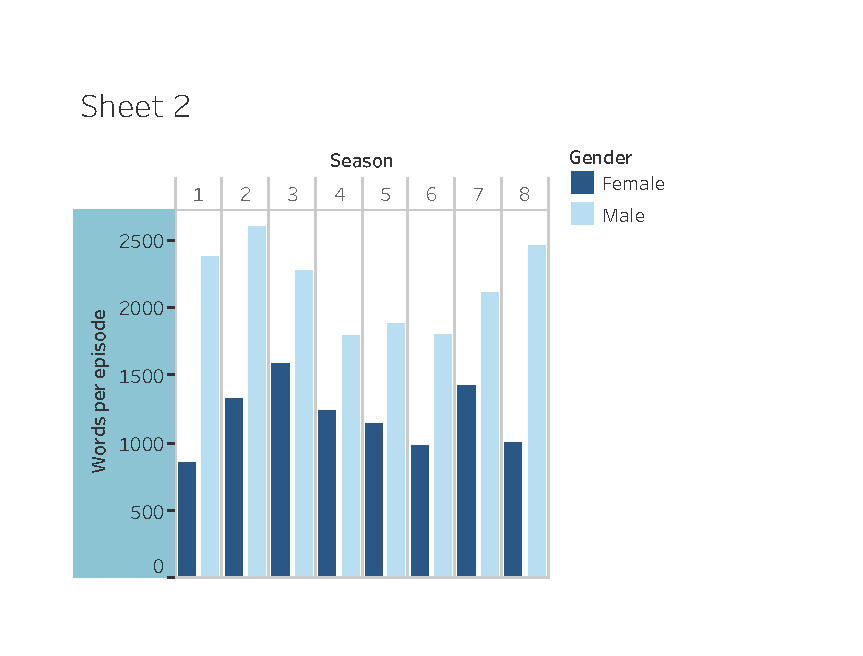
\includegraphics[width=0.9\textwidth]{fig/got}
\end{frame}

\begin{frame}{Workflow}
	\begin{enumerate}
		\item Formulate research question
		\item Collect data
		\item Pre-process data
		\item Analyze data
		\item Draw conclusions
	\end{enumerate}

	\pause
	\dots programming is useful for steps 2--4
\end{frame}



\begin{frame}{Summary}
	\begin{itemize}
		\item 
	\end{itemize}
\end{frame}

\end{document}
